%
% fourier.tex
%
% (c) 2025 Prof Dr Andreas Müller
%
\documentclass[tikz]{standalone}
\usepackage{amsmath}
\usepackage{times}
\usepackage{txfonts}
\usepackage{pgfplots}
\usepackage{csvsimple}
\usetikzlibrary{arrows,intersections,math}
\begin{document}
	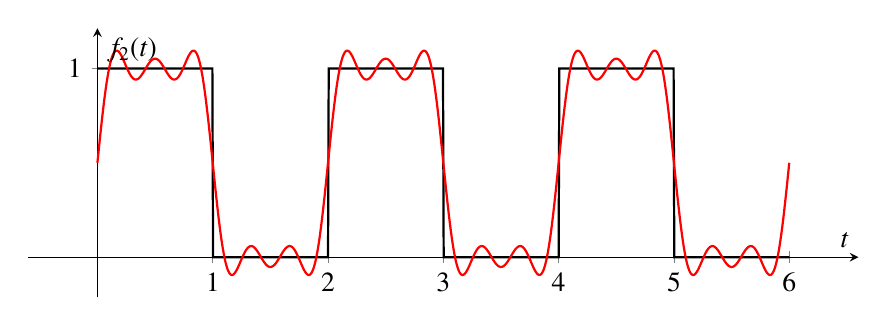
\begin{tikzpicture}
		\begin{axis}[
			axis lines = middle,
			xlabel = {$t$},
			ylabel = {$f_2(t)$},		
			domain=0:6,
			samples=1000,
			xtick={0,1,2,3,4,5,6},
			ytick={0,1},
			enlargelimits,
			width=\textwidth,
			height=5cm
			]
			\addplot[thick] {mod(floor(x),2) == 0 ? 1 : 0};
			\addplot[red, thick] {(1/2) + 
				(2/pi)*sin(pi * deg(x)) + 
				(2/(3*pi))*sin(pi *3*deg(x)) +
				(2/(5*pi))*sin(pi *5*deg(x))};
		\end{axis}
	\end{tikzpicture}
\end{document}
